\chapter{From edges to contours} % - Current State-of-the-Art}
\label{Chapter3}
\settocdepth{subsection}

In this chapter we review a recent segmentation method, introduced in \cite{Arbelaez09} and further developed %described, refined 
in \cite{Arbelaez11}. The algorithm is known as {\tt gPb-OWT-UCM}, after the three stages of its pipeline. We used it to illustrate segmentation concepts in \sref{sec:ch1-segmentation-terminology}. As you can see in \fref{fig:gPb-OWT-UCM-high-level}, the method incorporates a self-sufficient edge detector - {\tt gPb} \cite{Maire2008using}. The output of the detection is further processed to yield contours at multiple scales by %, in effect 
providing a hierarchical segmentation in an {\tt UCM} \cite{Arbelaez2006boundary}.

\begin{figure}[ht!]
\centering
 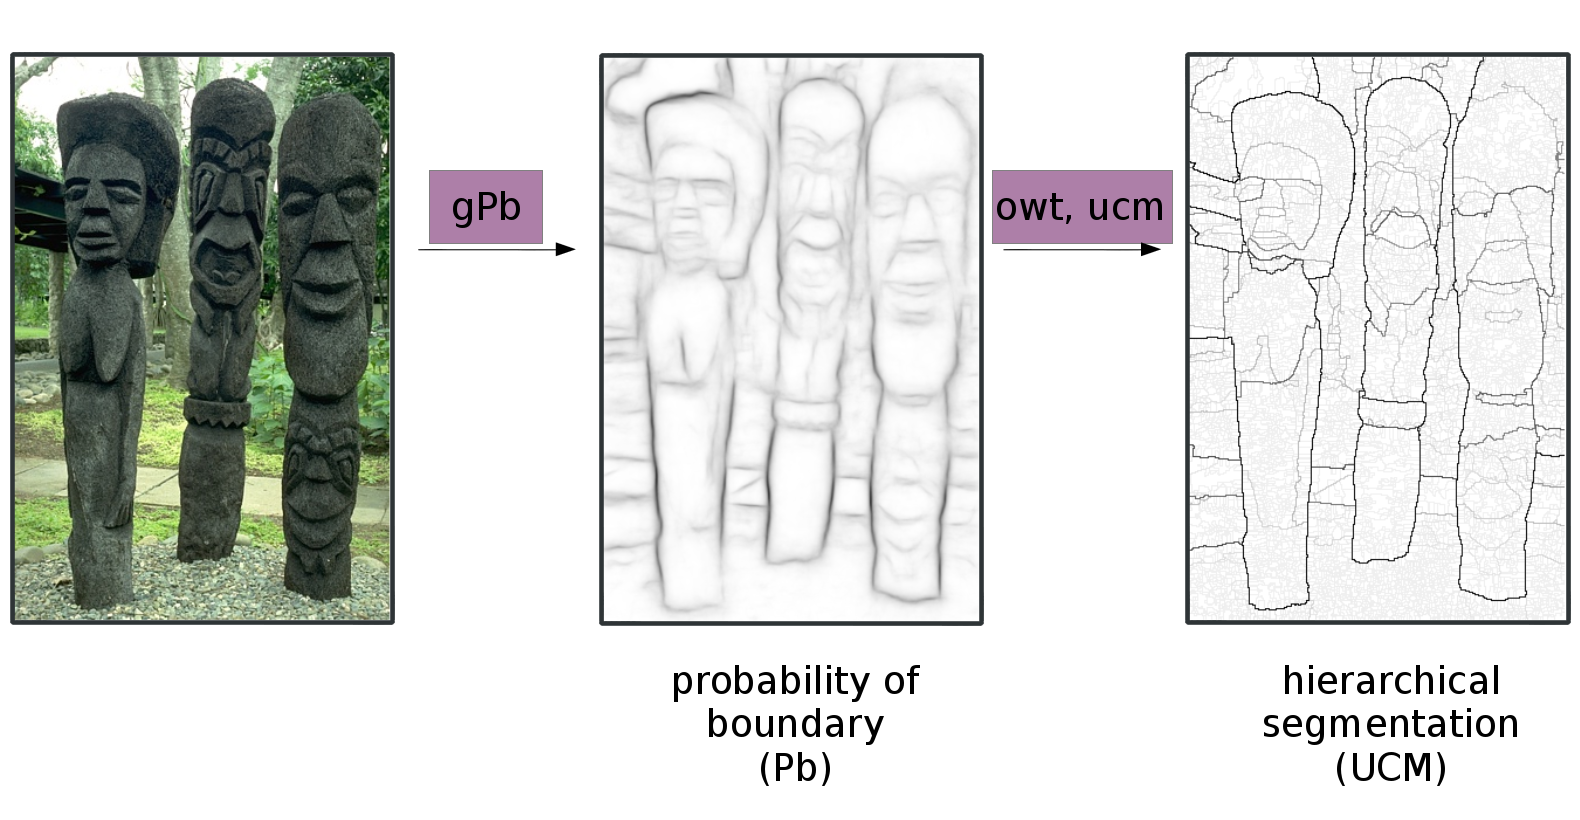
\includegraphics[width=1\textwidth]{images/gPb-OWT-UCM/gPb-OWT-UCM-high-level.png}
\caption[High-level view of the {\tt gPb-OWT-UCM} algorithm]{High-level view of the {\tt gPb-OWT-UCM} - a segmenter that first extracts edges and subsequently uses them to obtain a multiscale segmentation.}
\label{fig:gPb-OWT-UCM-high-level}
\end{figure}

{\tt OWT-UCM}, as we remarked in the review of the state-of-the-art detectors and segmenters in \sref{sec:ch1-focus-SoA-methods}, is the current method of choice for edge detectors which want to provide {\bf %closed 
contours} in addition to edges.

In this chapter we review {\tt gPb-OWT-UCM}, focusing mostly on the edges-to-contours part of the pipeline ({\tt OWT-UCM}). We discuss limitation of this approach and in \cref{Chapter4} propose an alternative solution for obtaining a hierarchy of closed contours from a non-oriented {\tt Pb} edge signal.

\section{{\tt gPb-OWT-UCM} algorithm pipeline}
\begin{figure}[ht!]
\centering
 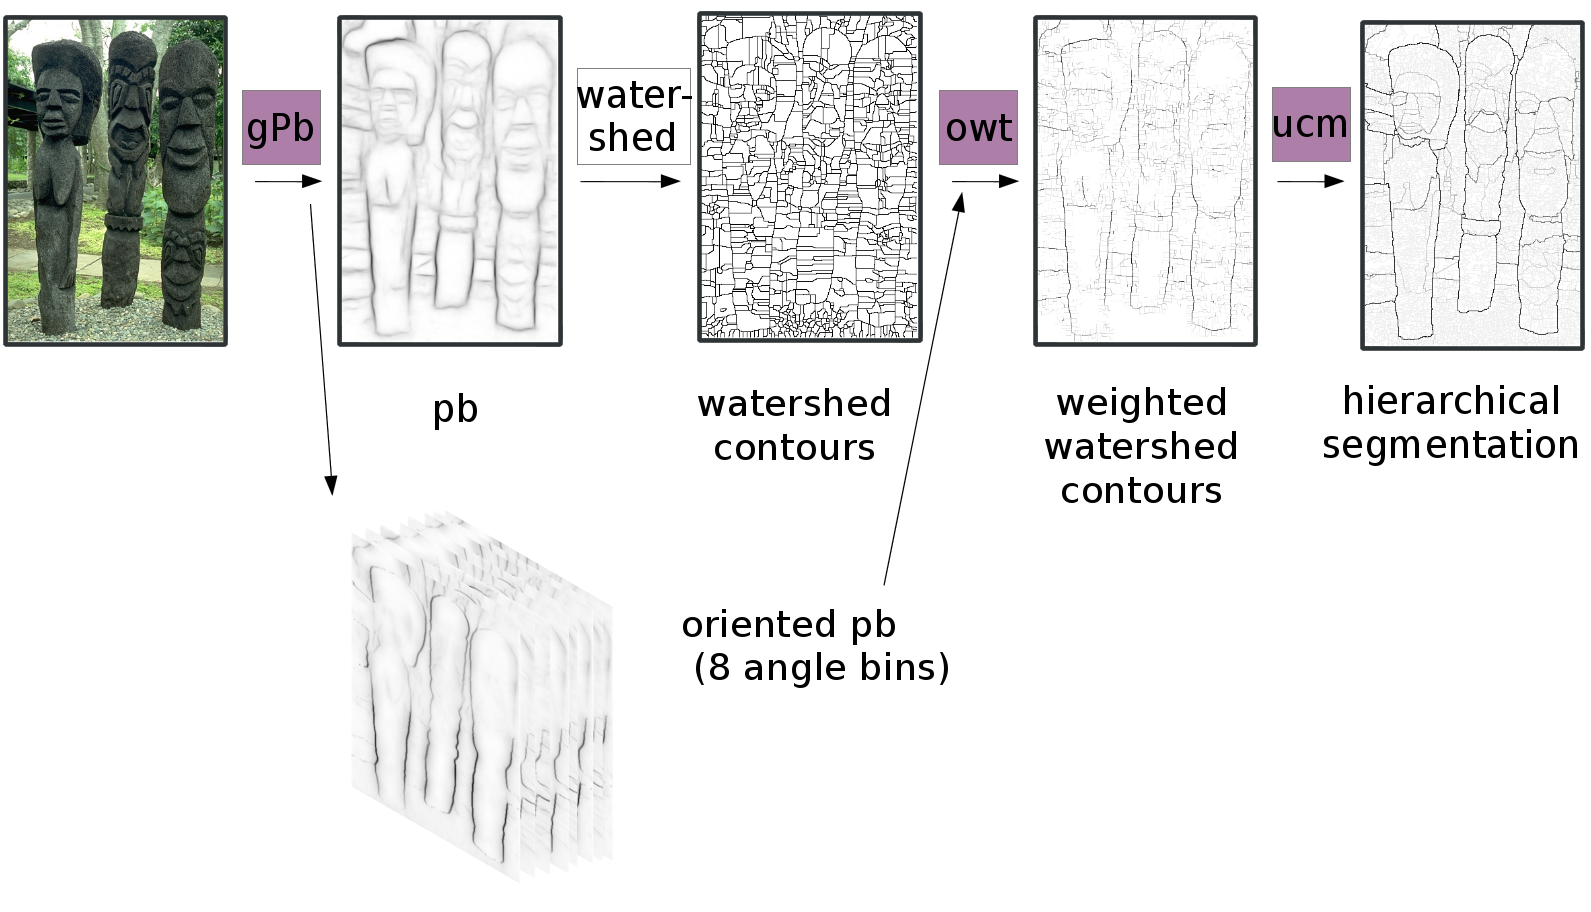
\includegraphics[width=1\textwidth]{images/gPb-OWT-UCM/gPb-OWT-UCM_pipeline.png}
\caption[{\tt gPb-OWT-UCM} detailed pipeline]{{\tt gPb-OWT-UCM} detailed algorithm pipeline. We are explicitly including the ``watershed transform'' operation and its output - watershed contours, as it is crucial both to this technique (to be described in \sref{sec:ch3-watershed}) and to our method, which we propose in \cref{Chapter4}. Notice how {\tt OWT} requires as input an {\bf oriented boundary signal} $oPb(x,y,\theta)$, which the {\tt gPb} edge detector provides.}
\label{fig:gPb-OWT-UCM-pipeline}
\end{figure}

The {\tt OWT-UCM} has been advertised \cite{Arbelaez09} as a {\it generic} approach that would allow to obtain contours from {\it any} edge detection algorithm, while preserving boundary quality. As it can also be seen in the detailed pipeline in \fref{fig:gPb-OWT-UCM-pipeline}, this is not quite the case. %correct. 
The algorithm {\tt OWT} requires as its input from the detector %output to be 
an {\it oriented probability of boundary} $oPb(x,y,\theta)$ indicating the strength of the edge at pixel location $(x,y)$ with orientation $\theta$ (see also Section~\ref*{sec:ch2-alternative-capturing-context}~\ref{par:ch2-oPb}).

It is an {\bf objective of the current thesis} to offer a truly universally applicable approach, which can operate on non-oriented output of edge detectors ($Pb(x,y)$) to produce a hierarchical segmentation - {\tt UCM} (see \cref{Chapter4} for %an introduction to 
our proposal).

\subsection{First stage of the pipeline - edge detection} % gPb
\label{sec:ch3-gPb}
The {\tt Pb} edge detector \cite{Martin2004learning} utilises local cues - colour, brightness, and texture, to judge for the presence of a boundary. 

The {\tt gPb} algorithm \cite{Maire2008using} takes this idea further. The features built in {\tt Pb} are globalised using spectral clustering. Multiple-scale approach gives competitive edge detection results. \fref{fig:gPb-algorithm-details-mPb_sPb_gPb} gives details on the edge detection part of the {\tt gPb-OWT-UCM} pipeline - {\tt gPb}.

\subsubsection{{\tt Pb} - a quantised oriented probability of boundary}
The {\tt Pb}  algorithm computes for each pixel location in an image, local image features from gradients for {\bf 8 orientations}. 

\paragraph{The features:} 4 feature channels are employed in this method. Colour is represented using the \textit{CIE L*a*b* (CIELAB)} colour space \cite{Hoffmann2003cielab}, since the distance between the points in a local neighbourhood is perceptually meaningful. % distance between points in CIELAB space is perceptually meaningful in a local neighbourhood
In addition to {\it brightness (L)}, {\it colour a}, and {\it colour b}, {\it textons} are also utilised.


\paragraph{Gradient magnitude:} Gradients at 8 orientations $\theta$ for each of the 4 feature channels are computed. The gradient signal is obtained by finding the {\bf distance} % chi-square distance
between histograms of the two halves (determined by $\theta$) of a local patch. This allows to associate a score to each pixel location (the ``gradient magnitude'').

% TODO how do we obtain a score for each pixel location
% from \cite{Arbelaez11}
%- For each half-disc, we histogram the intensity values of the pixels of I covered by it. The gradient magnitude G at location (x;y) is defined by the $\chi^2$ distance between the two half-disc histograms g and h. ...
%-  This computation is motivated by the intuition that contours correspond to image discontinuities and histograms provide a robust mechanism for modelling the content of an image region. A strong oriented gradient response means that a pixel is likely to lie on the boundary between two distinct regions.

\paragraph{Cue combination:} Effective combination of these multiple features % oriented gradient magnitude signals 
is essential. To this end, a simple weighted linear combination proves sufficient. The weights for the % individual 
cues are learnt in a supervised manner, by % training a %binary % TODO is it binary?
%logistic regression 
%classifier 
using human-labelled ground-truth boundaries (the dataset used is BSDS300; for details and an example of its updated version, which we utilise, see \sref{sec:ch5-BSDS500-dataset} and \fref{fig:BSDS-annotations}). 

In effect, a posterior oriented Pb $oPb(x,y,\theta)$ is obtained, indicating for each pixel the strength of the boundary through the centre of the local feature patch.

\subsubsection{{\tt mPb} - features at multiple scales}
\label{sec:ch3-mPb}

{\bf Coarse-to-fine} is a powerful concept in computer vision \cite{Ren2008multi}. It is employed in the {\tt mPb} part of the edge detector to allow to capture the salient edges {\bf at different scales}. Each of the features considered is computed at 3 different scales, \ie, for patches of 3 different sizes centred around the pixel location. This technique permits % allows 
to extract more edges.

So for each of the local features, an oriented gradient operator is computed at {\bf 3 scales} and for {\bf 8 orientations}. As for {\tt Pb}, the channels are combined linearly, yielding $mPb(x,y,\theta)$.

%- In contrast to [2] and [28], which use a logistic regression classifier to combine cues, we learn the weights by gradient ascent on the F-measure using the training images and corresponding ground truth of the BSDS.

\begin{figure}[ht!]
\centering
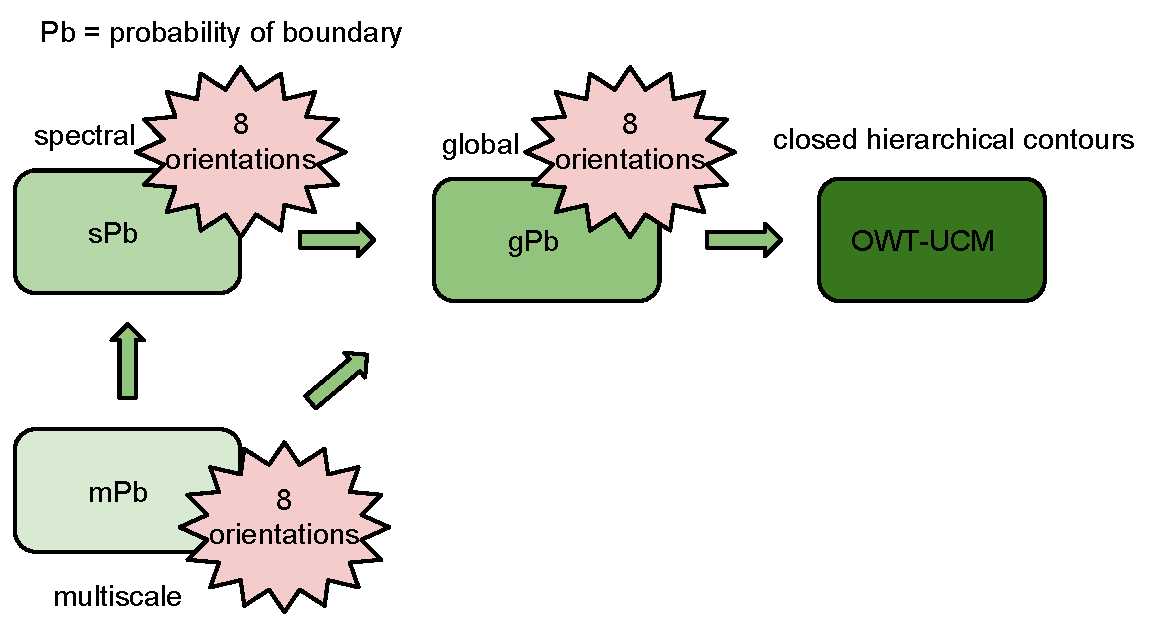
\includegraphics[width=1\textwidth]{images/gPb-OWT-UCM/gPb-algorithm-details-mPb_sPb_gPb.pdf}
\caption[{\tt gPb-OWT-UCM} pipeline with focus on the edge-detection stage - {\tt gPb}]{{\tt gPb-OWT-UCM} pipeline with focus on the edge-detection stage. The {\tt gPb} combines the results of the two edge detectors - {\bf multiscale} and {\bf spectral}.}
\label{fig:gPb-algorithm-details-mPb_sPb_gPb}
\end{figure}

\subsubsection{{\tt sPb} - globalisation through spectral clustering}
% A non-oriented signal - the strength of the boundary can be computed by taking the maximum per orientation:
% \[
%  mPb(x,y)=\max_{\theta} mPb(x,y,\theta)
% \]
% NOTE and so what? :D

Spectral clustering is a technique often employed for image segmentation, among others. Details on it are given in \cite{Leung1998contour,Shi2000normalized,Fowlkes2003learning,Fowlkes04}, here we only provide the key %most relevant 
points for the %gist 
{\tt sPb} detector, which is based on % inspired
spectral clustering. 

A sparse, symmetric affinity matrix $W$ is built using the {\tt mPb} signal. The matrix expresses the inter-pixel similarities for pixels not further from each other than a fixed radius $r=5$ pixels. Pixels separated by a strong boundary have low affinity.

% TODO not quite?!?!
% The maximum per gradient orientation of the local cues computed at each location in the image define a matrix of inter-pixel similarities. 

A generalised eigenproblem is derived for the affinity matrix $W$. The {\bf generalised eigenvectors contain edge information}. %Simply clustering % K-means in N-Cuts
% them to obtain the edges would introduce artefacts - uniform regions (\eg sky, grass) would be erroneously subdivided. Instead, the 
The {\bf gradients} %  convolve with Gaussian directional derivative filters at multiple orientation \theta
(for 8 orientations, quantised as before) of the first 16 %few 
of them %eigenvectors 
are combined in a {\bf soft manner} (a weighted linear combination) % weights are derived from the eigenvalues 
to produce the oriented spectral edge detector $sPb(x,y,\theta)$.

\subsubsection{{\tt gPb} - a combination of {\tt mPb} and {\tt sPb}}
\label{sec:ch3-Pb_mPb_sPb_gPb}
As we just learnt, {\tt mPb} detector fires at all edges. {\tt sPb}, being a spectral method, fires only at salient edges \cite{Fowlkes04,Yu2005segmentation}. {\tt gPb} provides a simple way to combine the two results, see also \fref{fig:gPb-algorithm-details-mPb_sPb_gPb}. The weights $\alpha$ and $\beta$ for the {\bf linear combination} 
\[
 gPb(x,y,\theta)=\alpha \cdot mPb(x,y,\theta) + \beta \cdot sPb(x,y,\theta)
\]
are learnt on the training subset of BSDS500 \cite{BSDS500resources} (similarly to the learning of the weights for the local cues combination). % the weights are learned by gradient ascent on the F-measure using the BSDS training images.

\paragraph{Performance comparison of the {\tt gPb} components:} 
\label{par:ch3-Pb_mPb_sPb_gPb}
\fref{fig:Pb_mPb_sPb_gPb} shows a performance comparison of the sub-algorithms comprising the {\tt gPb} detector. 

Details on the evaluation metric are to be given in \sref{sec:ch5-BPR-evaluation-metric}. For now it suffices to know that better methods occupy the upper right corner of the plot. Humans ``fail'' to achieve %reach 
a perfect score as the dataset contains multiple annotations. Hence, the human score represents their average agreement (calculated in an one-vs.-rest manner). 

Note how the single scale {\tt Pb} is ``missing'' high recall in comparison to {\tt mPb}, which computes each of the features at 3 different (channel-specific) scales. 

As the eigenvectors correspond to the most prominent of edges, the {\tt sPb} provides for higher precision (at the expense of recall). 

{\tt gPb} successfully benefits from the better of the two algorithms {\tt mPb} or {\tt sPb} in their respective superior regime.

\begin{figure}[ht!]
 \centering
 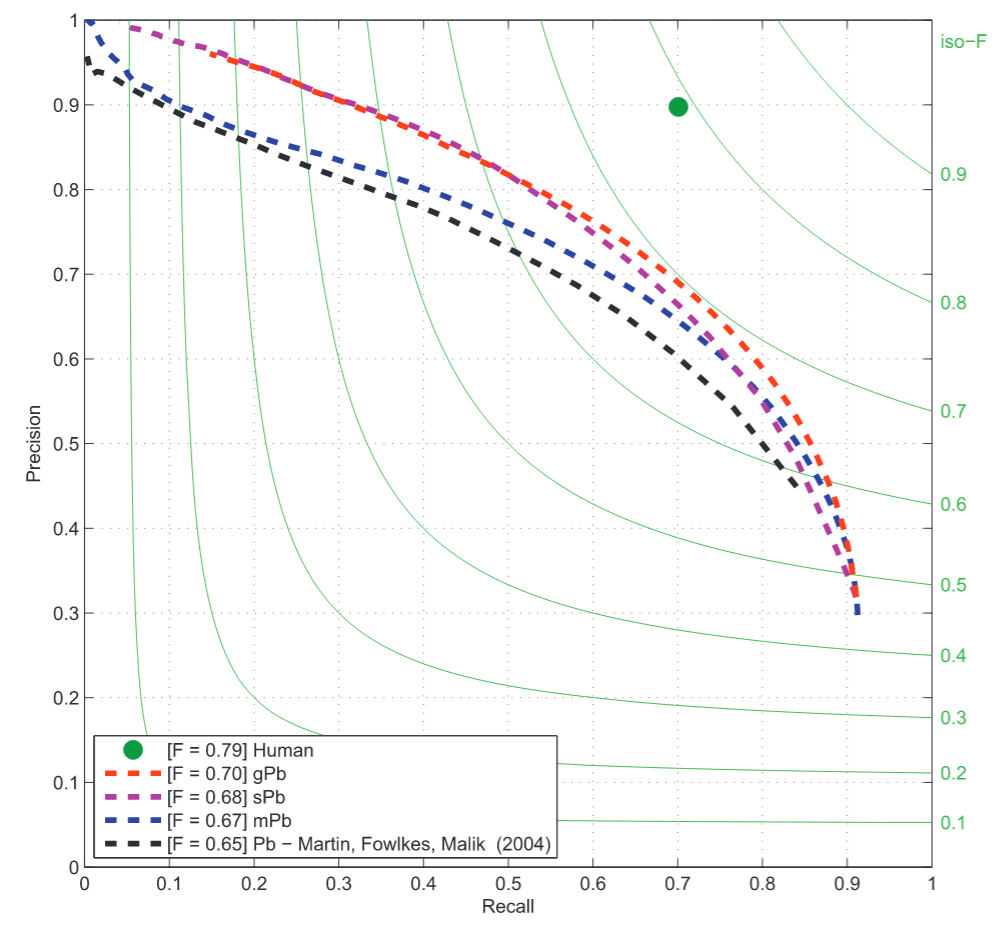
\includegraphics[width=0.6\textwidth]{images/gPb-OWT-UCM/Pb_mPb_sPb_gPb.png}
 \caption[{\tt gPb} evolution - plot results on the BSDS500 benchmark.]{{\tt gPb} evolution - evaluation results on the BSDS500 benchmark. See the text for details. Plot courtesy of \cite{Arbelaez11}.}
 \label{fig:Pb_mPb_sPb_gPb}
\end{figure}

In our own experiments described in \cref{Chapter5}, we will use similar reasoning to compare a method employing spectral clustering to one which does not use globalisation, see \sref{sec:ch5-SE_sPb-OWT-UCM}.

\subsection{Second stage of the pipeline - weighting the watershed} % OWT
The key idea for the last two stages %phases 
of the pipeline - {\tt OWT-UCM}, is that weighted watershed contours can be converted into a hierarchical segmentation.

\subsubsection{Watershed}
\label{sec:ch3-watershed}
% TODO
% from Marco's blog
%- The Watershed transformation considers the gradient magnitude of an image as a topographic surface. Pixels having the highest gradient magnitude intensities (GMIs) correspond to watershed lines, which represent the region boundaries. Water placed on any pixel enclosed by a common watershed line flows downhill to a common local intensity minima (LMI). Pixels draining to a common minimum form a catchment basin, which represent the regions.

As we mentioned in \sref{sec:ch1-watershed-transform}, the watershed transformation is used to obtain a segmentation from an intensity image. 
For a greyscale image, the gradient magnitude is used as a {\bf topological surface}. The {\tt gPb-OWT-UCM} algorithm takes instead the {\bf maximum edge signal} along the 8 orientations $\mathbf{gPb(x,y)}=\max\limits_{\theta}gPb(x,y,\theta)$. 

\paragraph{The watershed transformation:} If we think of rain falling on the %is placed on 
topological surface, all pixels that ``drain'' to a common local minimum form a catchment basin - these are the {\it watershed regions (segments)}. The boundaries of the regions are the watershed \textit{pixels} (\textit{contours}). 
% Given an intensity %a greyscale 
% image as an input, it would output watershed \textit{segments} (\textit{regions}), which are complimentary % complimentary :D
% to the watershed \textit{pixels} (\textit{contours}). 
The latter are by construction closed contours. 

Alternative way to understand the operation is by imagining ``water'' flooding the topological surface from all the local minima. The {\it watershed contours} are the locations where ultimately the separate basins will meet.

\fref{fig:watershed-transformation-forming-regions} shows a toy example illustrating how the regions are formed.
%- The figure below depicts how the regions are found. (a) is a matrix showing typical GMI values with the LMIs circled. (b) shows the morphological gradient directions for the matrix in (a).

\paragraph{Output of the watershed transformation:} A well-known shortcoming of the watershed transform is that the 
segmentation produced by it is an {\bf oversegmentation}, due to a catchment basin forming around every regional minimum.

%- A major problem with this method is that it very often results in severe over segmentation, such as in the segmentation below. There have been several attempts at overcoming this problem. Meyer and Beucher proposed a marker-controlled strategy. Markers are placed on the image to represent objects. The Watershed transformation is then run by flooding from the markers. This requires prior knowledge of the objects in the image or even manual input.


\begin{figure}[ht!]
 \centering
 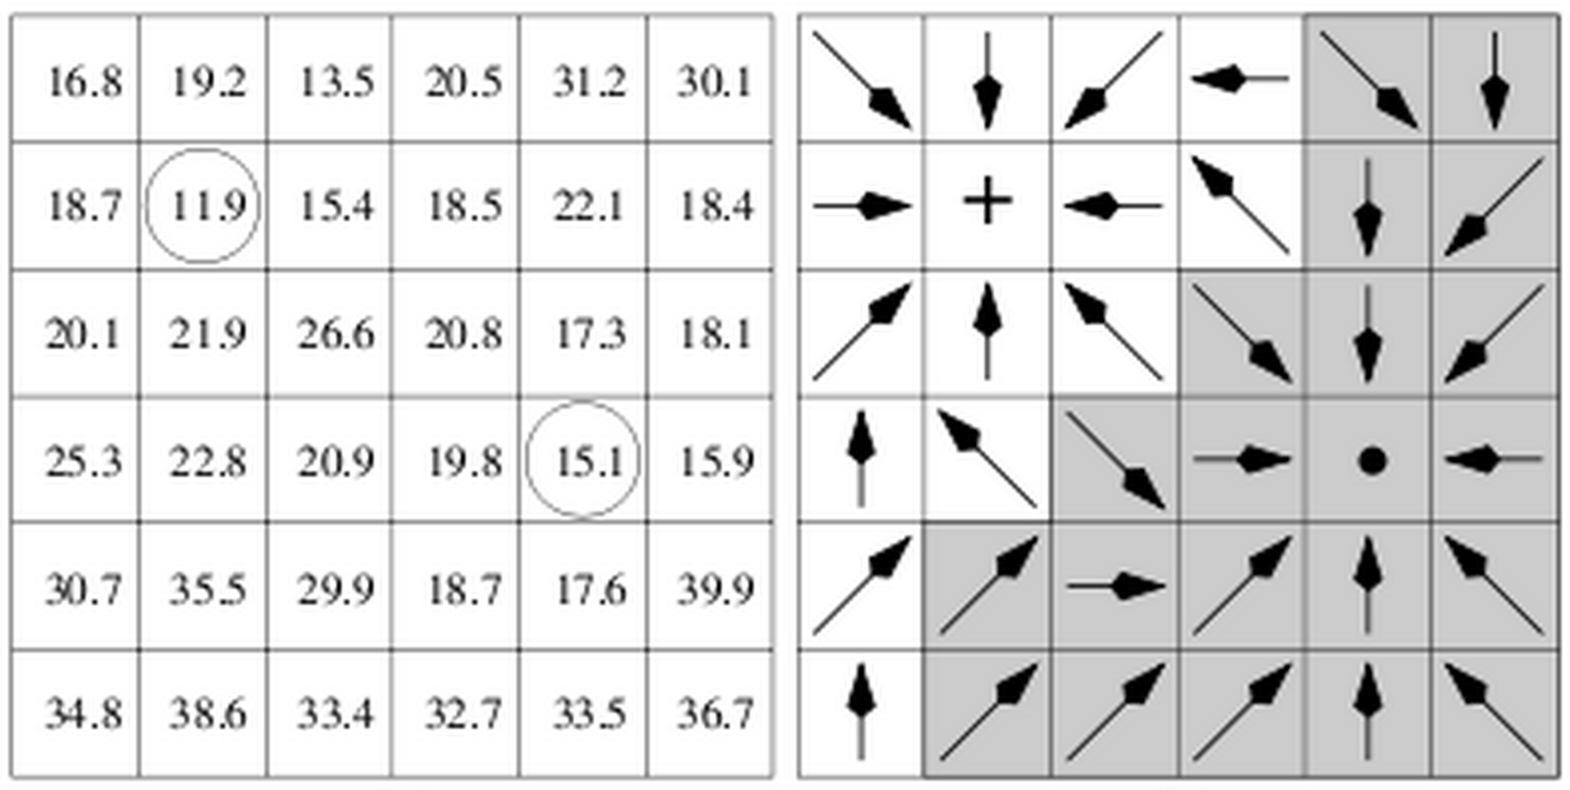
\includegraphics[width=0.5\textwidth]{images/gPb-OWT-UCM/watershed-transformation-forming-regions.png}
 \caption[Watershed transformation - forming the regions]{Watershed transformation - forming the regions. {\bf Left:} the topological surface, with the local minima circled (8-neighbourhood is used. % in {\tt OWT}).
 {\bf Right:} The morphological gradient directions, which determine the regions (for the surface on the left). Courtesy of \cite{MarcoBlog2007Watershed}.}
 \label{fig:watershed-transformation-forming-regions}
\end{figure}

Note that the watershed algorithm only provides a {\bf single segmentation}, but does not build a hierarchy. %but not weights to them, hence, 
Najman~\etal \cite{Najman1996geodesic} offer a way to obtain a hierarchy of segmentations from the watershed pixels, which unfortunately involves the selection of a {\bf set of markers}.

Unlike ``Seeded region growing'' \cite{Adams1994seeded}, the watershed algorithm does {\bf not require} as input any initial seeds for forming watershed regions. The local minima are trivially (automatically) obtained by applying a filter of size $3\times 3$ pixels on the topological surface.

\paragraph{Why is it useful?} The watershed transformation is a suitable intermediate {\bf step in obtaining hierarchical segmentation} from edge detection output, since it provides a straightforward means to close contours. The probability of boundary ({\tt gPb} here, and {\tt SE} in our experiments - in Chapters \ref{Chapter4} and \ref{Chapter5}) is a one-channel image and can therefore be used as an input to the watershed transformation. The result is a binary image which constitutes a segmentation. Thus, the watershed contours indicate all possible edge locations - the highest level of recall in the context of the Precision-Recall framework of~\cite{Arbelaez11} (see \sref{sec:ch5-BPR-evaluation-metric}). % (c.f. edge map)

In practice the vanilla watershed implementation in MATLAB \cite{MATLABwatershed} is used, with 8-connected neighbourhood for the regions.

\settocdepth{section}
\subsubsection{Oriented watershed transform ({\tt OWT})}
\settocdepth{subsubsection}
\label{sec:ch3-OWT}
So far %As they are, 
the watershed contours are unweighed, and provide only one segmentation - the trivial oversegmentation. To obtain hierarchical segmentation, we must {\bf weight} each contour, so that its value corresponds to its saliency. %of the underlying boundary. 

Na\"{\i}vely copying the value from the $gPb(x,y)$ signal as a score to the watershed contours produces artefacts (see \fref{fig:OWT_Arbelaez11}). In the proximity of strong boundaries, other weaker boundaries are scored higher, since their shape and orientation are not taken into account. Hence, the score from strong boundaries ``bleeds'' into their vicinity.

Arbel\'aez \etal solve this problem using the oriented boundary signal that they have obtained from the edge detector - $gPb(x,y,\theta)$. 

\paragraph{Watershed arc}\mbox{}\\\mbox{}\\
\label{par:ch3-watershed-arc}
The initial watershed region boundaries are poorly approximated by straight lines - their shape is too complex for this. 
Watershed arcs are recursively subdivided region boundaries, purpose being to simplify the shape until it can be approximated with a {\it line segment}. To help understand the concept, we first show an example for subdivision of edges.

\subparagraph{Subdivision of edges}\mbox{}\\\mbox{}\\
Maire \etal \cite{Maire2008using} applied the idea of an approximation %of a boundary 
with a line first to {\bf edges} in order to facilitate the localisation of junctions (and thus ``close'' contours). \fref{fig:Maire08using-contour-subdivision} shows a few edge fragments in a local image patch and (overlaid) their {\it line segment} approximations.

\begin{figure}[ht!]
 \centering
 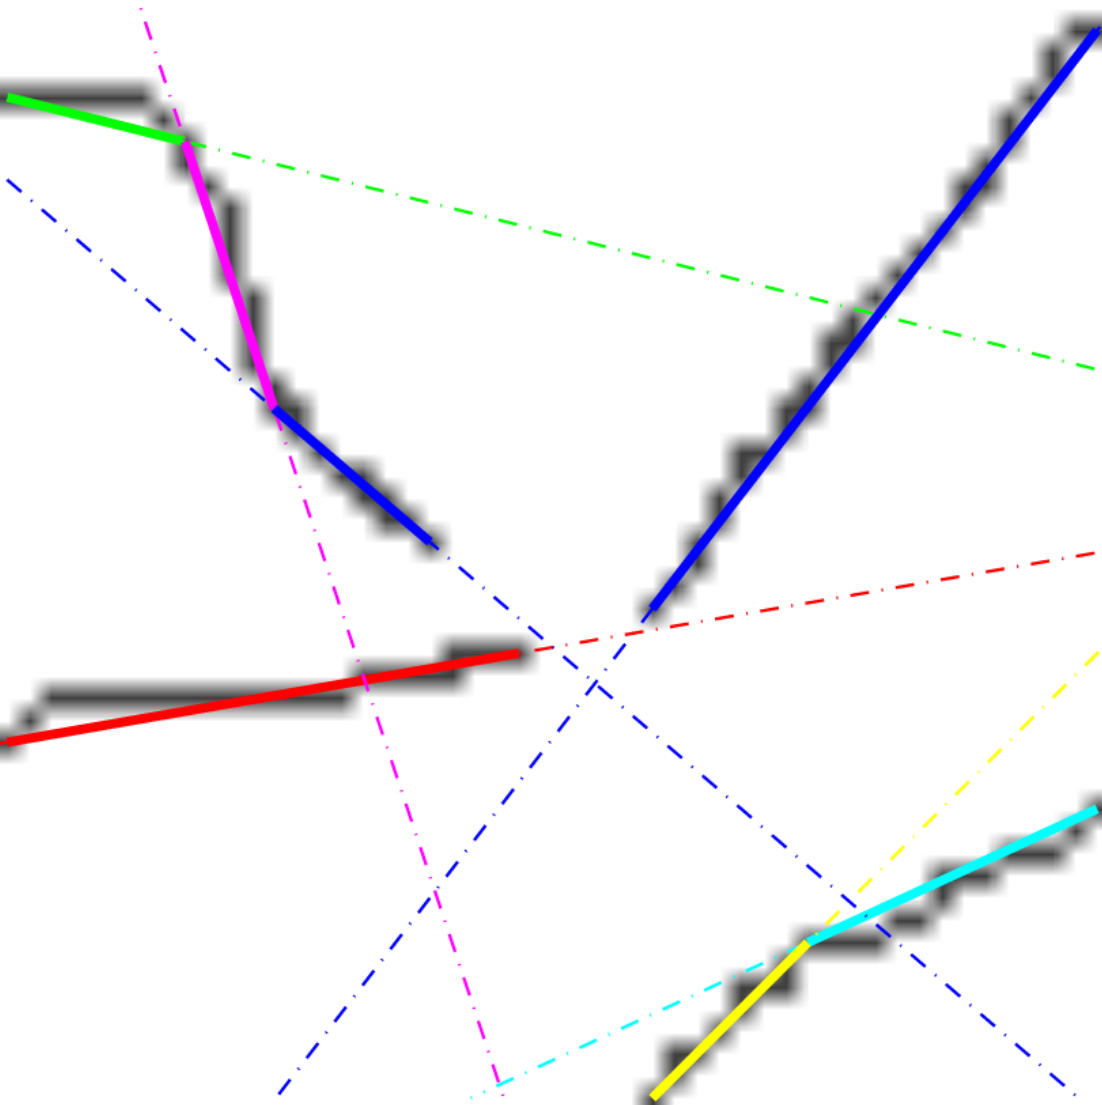
\includegraphics[width=0.4\textwidth,frame]{images/gPb-OWT-UCM/Maire2008using-contour-subdivision.png}
 \caption[Edges subdivision - an image patch]{{\bf Edges subdivision} into approximating linear pieces (the solid line segments). The intersections of the underlying straight lines (dashed and dotted line) would serve for junction detection. Courtesy of~\cite{Maire2008using}.}
 \label{fig:Maire08using-contour-subdivision}
\end{figure}

\subparagraph{Subdivision of region boundaries}\mbox{}\\\mbox{}\\
The above scheme is easily transferable to {\bf watershed contours}. The procedure is as first described in ``From contours to regions: An empirical evaluation'' \cite{Arbelaez09}. The {\bf watershed arcs} are recursively subdivided boundaries of watershed regions. An arc is split at an internal point which is maximally distant from the straight line through % connecting 
its endpoints. The {\it subdivision} is scale-invariant: the process stops when the maximal distance from an arc point to the {\it line segment} approximating it becomes smaller than a fixed fraction of the latter's % its %the segment's 
length. See also \fref{fig:Arbelaez11-contour-subdivision}.

\begin{figure}[ht!]
 \centering
 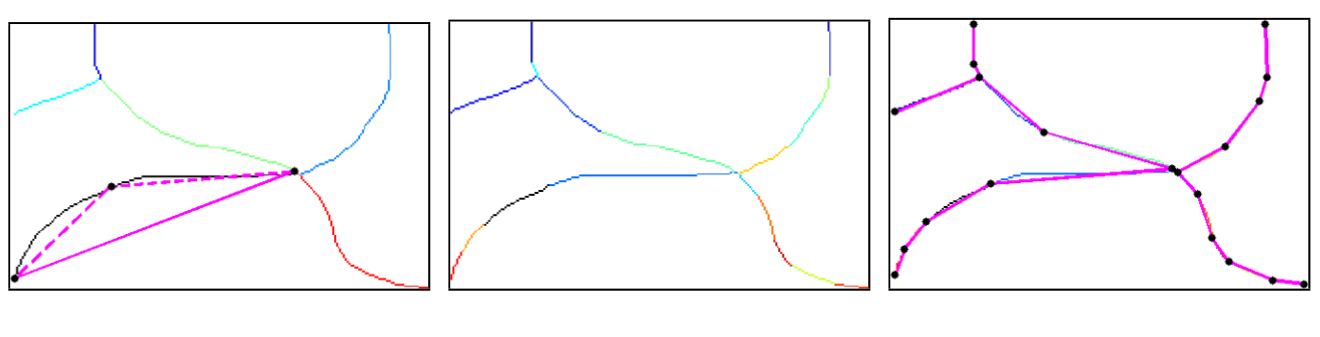
\includegraphics[width=1\textwidth]{images/gPb-OWT-UCM/Arbelaez11-contour-subdivision.png}
 \caption[Region boundary subdivision]{{\bf Region boundary subdivision} (courtesy of~\cite{Arbelaez11}). {\bf Left:} Colour-coded are given the initial watershed arcs - the entire  %full 
 region boundaries. Magenta solid line denotes the line approximation of the arc. A subdivision (to the farthest point on the arc) is indicated with two magenta dashed lines. {\bf Middle:} The final set of watershed arcs. A {\bf region boundary consists} therefore {\bf of one or more arcs}. {\bf Right:} The middle image, with the arc-approximating lines (magenta solid) overlaid.}
 \label{fig:Arbelaez11-contour-subdivision}
\end{figure}

\paragraph{{\tt OWT}:}
Now that the watershed arcs provide a sufficient simplification by subdividing a region boundary, an approximate orientation $\mathbf\theta$ can be assigned to each arc. The score to associate with each pixel on this arc is taken from the corresponding oriented boundary $gPb(x,y,\mathbf{\theta})$. Finally the scores from the watershed pixels are {\bf averaged per region boundary} (see \fref{fig:OWT_Arbelaez11} {\bf Left} and {\bf Far right}). 
By taking orientation into consideration, the {\tt OWT} reduces inaccurate high scores in the proximity of strong edges.

\begin{figure}[ht!]
 \centering
 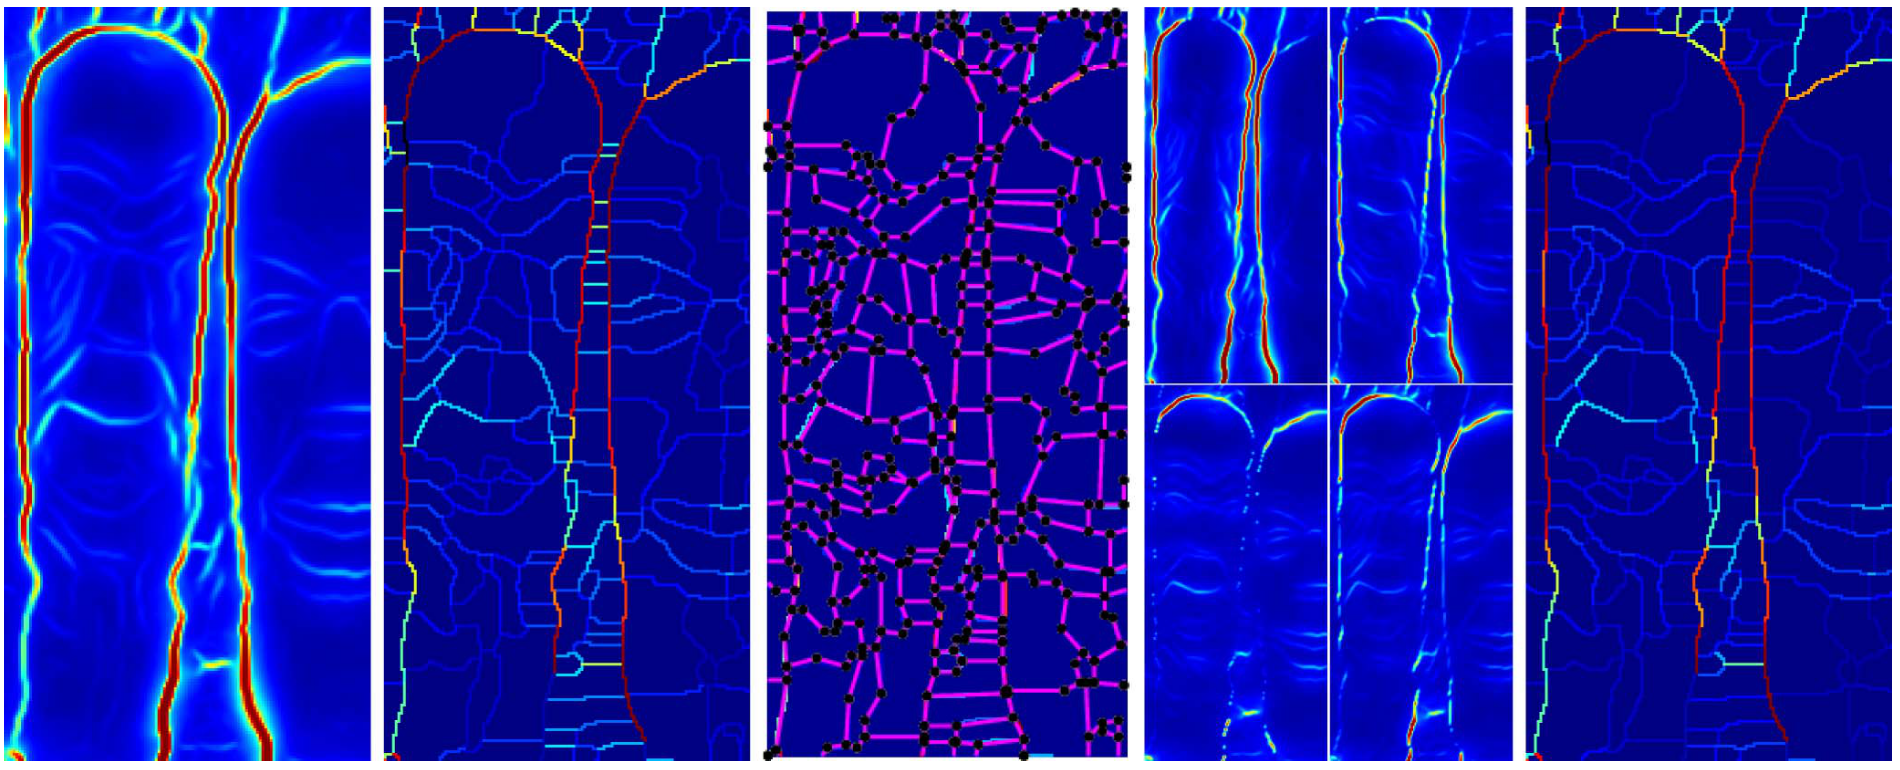
\includegraphics[width=1\textwidth]{images/gPb-OWT-UCM/OWT_Arbelaez11.png}
 \caption[{\tt OWT} compared to na\"{\i}ve value transfer]{{\tt OWT} compared to na\"{\i}ve value transfer (courtesy of~\cite{Arbelaez11}). {\bf Far left:} The maximal boundary strength across orientations $gPb(x,y)$. {\bf Left:} Na\"{\i}ve approach creates artefacts (see erroneously split region between statue's heads). {\bf Middle:} Subdivision of region boundaries into arcs. Magenta lines are the approximating {\it line segments}. {\bf Right:} $gPb(x,y,\theta)$ for 4 different $\theta$; 8 are used in practice. {\bf Far right:} {\tt OWT} leads to a reduction in artefacts close to strong boundaries.}
 \label{fig:OWT_Arbelaez11}
\end{figure}


\subsection{Third stage of the pipeline - {\tt UCM}}
\label{sec:ch3-UCM}
The {\it Ultrametric contour map} ({\tt UCM}) was introduced in \cite{Arbelaez2006boundary}. It constitutes a convenient data structure for the representation of a hierarchical segmentation, as we hinted in the introductory \cref{Chapter1}. 

The map is constructed by agglomerative clustering of regions based on the {\bf weight of their common boundary}. As {\tt OWT} produces weighted watershed contours where all pixels on the region boundary have the same weight, those weights are sorted and region merging is performed from the weaker to the stronger region boundaries. After merging two segments, their common boundary is removed, and a valid segmentation of the original image can be obtained.

The {\tt UCM} data structure represents a tree, at the leaves of which are the superpixels at the highest level of detail. Going up the tree ``merges'' regions and provides a coarser segmentation. At the root of the tree is a single segment which encompasses the whole image. The {\tt UCM} can also be understood as a real-valued image (see Figures \ref{fig:sub:segmentation-ucm} and \ref{fig:sub:segmentation-ucm-cc}) in which every region boundary is weighted by its scale of disappearance.

% TODO give the algorithm in an appendix

\section{Limitations of {\tt gPb-OWT-UCM}} %quantisation} % or drawbacks, don't say 'flaws'
\textbf{Low speed at test time:} One undeniable % undoubted, unquestionable, indisputable
limitation of the {\tt gPb-OWT-UCM} method is that it is slow on detection. On the BSDS500 dataset the segmenter takes on average 200 seconds per image.

\textbf{Oriented signals:} %Quantisation:} 
Another issue has mostly to do with the concept of using quantisation per angle orientation to estimate the strength of the boundary, as well as the weights for the pixels on the watershed contours. % It is a crude substitute for an actual edge and therefore, incapable of capturing fine variations in the boundary shape.
It is a crude substitute for the actual image edge and misses on using the shape of the edge to capture fine variations in the boundary constitution. % structure, makeup, formation

\textbf{OWT-UCM is not very convenient for general segmentation based on edge detection:} The algorithm is in essence an elaborate pipeline that does not easily accommodate different edge detectors. It has as an intrinsic ingredient the oriented probability of boundary. Nevertheless, many algorithms (\eg \cite{Kisilev2013Learning,Arbelaez2014multiscale,Isola2014crisp,Hallman2014}) re-use the second and third stage of the {\tt gPb-OWT-UCM} pipeline to also obtain segmentation in addition to their extracted edges. They are then forced to provide oriented boundary signal $oPb(x,y,\theta)$. Whenever there is a mismatch between the angle quantisation, results are %reported to be
unsatisfactory % poor, bad, substandard, weak, mediocre, sub par, insufficient
- see Section~\ref*{sec:ch2-alternative-capturing-context}~\ref{par:ch2-oPb}.

In \cref{Chapter4} we propose a more coherent % logical and consistent
and principled approach, which has the potential of addressing the above issues. It makes use of the detailed structured information present in local image patches containing edges. By applying this local knowledge it dispenses with the computation of oriented gradient signals for a fixed number of orientations that is so prevalent in the {\tt gPb-OWT-UCM} pipeline.
